\documentclass[11pt,a4paper]{report}

\usepackage[utf8]{inputenc}
\usepackage{graphicx}
\usepackage{amsmath,amsfonts,amssymb}
\usepackage{booktabs}
\usepackage{hyperref}
\usepackage{siunitx}
\usepackage{geometry}
\usepackage{caption}
\usepackage{subcaption}
\usepackage{enumitem}
\usepackage{siunitx}

\geometry{margin=2.5cm}

% Paragraph formatting
\setlength{\parindent}{0em}
\setlength{\parskip}{0.6em}


\title{STEM Benchmark Test Report}
\author{STEM Development Team}
\date{\today}

\begin{document}

\maketitle
\tableofcontents
\clearpage

% -------------------------------------------------------
\chapter{Introduction}
% -------------------------------------------------------
This report documents the verification tests performed on the STEM.
The purpose is to validate numerical accuracy through comparison against
analytical solutions and established benchmark results.

Each chapter corresponds to a benchmark configuration, including a description
of the mathematical model, numerical setup, and comparison of results.

\clearpage
% ==============================================================================================
\chapter{Dynamic point load on elastic halfspace}\label{ch:pekeris}
% ==============================================================================================

% ----------------------------------------------------------------------------------------------
\section{Introduction}
% ----------------------------------------------------------------------------------------------
This benchmark compares the STEM numerical solution against the analytical solution
for a dynamic point load applied to the surface of an elastic half-space.

The analytical solution was derived by Pekeris and is detailed in~\cite{Verruijt_2010}.
The analytical solution provides closed-form expressions for the vertical displacement along the surface of the
half-space, enabling a direct time-history comparison against the numerical model.


% ----------------------------------------------------------------------------------------------
\section{Model Description}
% ----------------------------------------------------------------------------------------------

% ..............................................................................................
\subsection{Geometry, mesh and loading}
% ..............................................................................................
The point load was modelled in a three-dimensional domain representing an elastic half-space.
An overview of the geometry for the numerical analysis is shown in Figure~\ref{fig:3D_scheme}.
The soil has a width, length and depth of \qty{5}{\meter} and is subjected to a compressive pulse load, $F(t)$,
which is suddenly applied at the top edge:

\begin{equation}
    F(t) =
     \begin{cases}
    0, & \text{if } t<0\\
    \qty{-1000}{\kilo\newton}, & \text{if } t>0\\
    \end{cases}
\end{equation}


\begin{figure}
    \centering
    \includegraphics[width=0.75\textwidth]{pekeris/mesh.pdf}
    \caption{Geometry, mesh and loading conditions for the three-dimensional wave propagation problem.}
    \label{fig:3D_scheme}
\end{figure}

The soil is discretised in high-order tetrahedral elements with size \qty{0.15}{\meter}.
In total the model comprises 596~493~elements.

The nodes at the sides of the soil have absorbing boundaries at the free ends, and with fixed boundary conditions
on the perpendicular plane along the axis of symmetry.
At the bottom the soil is assumed to be fixed, simulating the existence of the top of bedrock that has a
significantly larger stiffness than the soil above.

% ..............................................................................................
\subsection{Materials and numerical parameters}
% ..............................................................................................
The soil is modelled as an one-phase continuum with a linear elastic constitutive law, with the
following parameters:

\begin{itemize}[noitemsep,topsep=0pt,parsep=0pt,partopsep=0pt]
    \item Young's modulus: \qty{30}{\mega\pascal},
    \item Poisson ratio: \qty{0.3},
    \item Density: \qty{2000}{\kilogram\per\meter\cubed}.
\end{itemize}

Material damping is included via Rayleigh damping, with parameters that provide a damping ratio of
\qty{0.01}{\percent} at \qty{1}{\hertz} and \qty{80}{\hertz}.

The dynamic analysis is performed over a \qty{0.20}{\second} time window, with a time step of \qty{0.001}{\second}.
The system of equations is solved using the Newmark time integration~\cite{Newmark_1959} scheme with
parameters $\beta = 0.25$ and $\gamma = 0.5$.

% ----------------------------------------------------------------------------------------------
\section{Results}
% ----------------------------------------------------------------------------------------------
Figure~\ref{fig:pekeris_results} presents the time histories of the vertical displacement for three
nodes. located at 1, 2 and~\qty{3}{\meter} from the load, located along the surface.
The figure compares the STEM results against the analytical solution.
If follows that there is an agreement between both solutions, demonstrating the accuracy of the STEM
for this type of dynamic loading condition.

\begin{figure}[h]
    \centering
    \includegraphics[width=0.8\textwidth]{pekeris/time_history.pdf}
    \caption{Comparison of the vertical displacement time histories at surface nodes located at:
     (a) \qty{1}{\meter}, (b) \qty{2}{\meter} and (c) \qty{3}{\meter} from the load.}
    \label{fig:pekeris_results}
\end{figure}

% ==============================================================================================
\chapter{Dynamic strip load on 2D elastic halfspace} \label{ch:strip_load_2D}
% ==============================================================================================

% ----------------------------------------------------------------------------------------------
\section{Introduction}
% ----------------------------------------------------------------------------------------------
This benchmark compares the STEM numerical solution against the analytical solution,
where a dynamic line load is applied along the surface of an elastic half-space discretised in a plane-strain setting.

The analytical solution is presented in~\cite{Verruijt_Brinkgreve_Li_2008}.
The analytical solution provides closed-form expressions for the vertical stress along the surface of the
half-space, enabling a direct time-history comparison against the numerical model.

% ----------------------------------------------------------------------------------------------
\section{Model Description}
% ----------------------------------------------------------------------------------------------

% ..............................................................................................
\subsection{Geometry, mesh and loading}
% ..............................................................................................
The soil domain is modelled in 2D and represents a \qty{20}{\meter} (x-direction) by \qty{10}{\meter}
(y-direction) soil layer, modelled with high-order triangular elements. The mesh uses an average
element size of \qty{1}{\meter}. Figure~\ref{fig:strip2d_mesh} illustrates the geometry and mesh
adopted for the analysis.

The strip load is applied at the surface with a width of \qty{1}{\meter}.
A downward line load with magnitude \qty{1e6}{\newton\per\meter} is applied instantaneously and kept
constant during the analysed time window:

\begin{equation}
    q(t) =
    \begin{cases}
        0, & t < 0, \\
        \qty{-1000}{\kilo\newton\per\meter}, & t \geq 0.
    \end{cases}
\end{equation}

The nodes at the bottom are fully fixed, while the two vertical sides are restrained only in the normal direction
(roller boundaries) to allow vertical and tangential movement.

\begin{figure}
    \centering
    \includegraphics[width=0.75\textwidth]{strip_load_2D/mesh.png}
    \caption{Geometry, mesh and boundary conditions for the dynamic strip load problem.}
    \label{fig:strip2d_mesh}
\end{figure}

% ..............................................................................................
\subsection{Materials and numerical parameters}
% ..............................................................................................
The soil is modelled as an one-phase continuum with a linear elastic constitutive law, with the
following parameters:

\begin{itemize}[noitemsep,topsep=0pt,parsep=0pt,partopsep=0pt]
    \item Young's modulus: \qty{30}{\mega\pascal},
    \item Poisson ratio: 0.2,
    \item Density: \qty{2000}{\kilogram\per\meter\cubed}.
\end{itemize}

Material damping is included via Rayleigh damping, with parameters that provide a damping ratio of
\qty{0.5}{\percent} at \qty{1}{\hertz} and \qty{80}{\hertz}.

The dynamic analysis is performed over a \qty{0.20}{\second} time window, with a time step of \qty{0.001}{\second}.
The system of equations is solved using the Newmark time integration~\cite{Newmark_1959} scheme with
parameters $\beta = 0.25$ and $\gamma = 0.5$.

% ----------------------------------------------------------------------------------------------
\section{Results}
% ----------------------------------------------------------------------------------------------
Figure~\ref{fig:strip2d_results} presents the vertical stress at a depth of {\qty{-1}{\meter}}
below the surface, at three moments in time: \qty{0.05}{\second}, \qty{0.075}{\second} and \qty{0.10}{\second}.
The figure compares the STEM results against the analytical solution.
If follows that there is an agreement between both solutions, demonstrating the accuracy of the STEM
for this type of dynamic loading condition.


\begin{figure}[h]
    \centering
    \includegraphics[width=0.8\textwidth]{strip_load_2D/time_history.pdf}
    \caption{Vertical stress at a depth of {\qty{-1}{\meter}} below the surface at three moments in time:
    (a) \qty{0.05}{\second}, (b) \qty{0.075}{\second} and (c) \qty{0.10}{\second}.}
    \label{fig:strip2d_results}
\end{figure}

\chapter{Dynamic strip load on 3D elastic halfspace}


% ----------------------------------------------------------------------------------------------
\section{Introduction}
% ----------------------------------------------------------------------------------------------
This document summarises the regression benchmark implemented in
\texttt{test\_strip\_load\_3D.py}. The problem extends the 2D strip load configuration to a
three-dimensional setting by extruding the plane-strain domain over \qty{1}{\meter} in the
out-of-plane direction. The aim is to confirm that the STEM modelling utilities correctly generate
the Kratos input deck, enforce the boundary conditions and recover the stored Linux reference
solution for a rapid surface loading event.


% ----------------------------------------------------------------------------------------------
\section{Model Description}
% ----------------------------------------------------------------------------------------------

% ..............................................................................................
\subsection{Geometry, Mesh and Loading}
% ..............................................................................................
The 3D model represents a \qty{20}{\meter} (x) by \qty{10}{\meter} (y) soil layer extruded to
\qty{1}{\meter} thickness in the z-direction, resulting in a prismatic block. Quadratic
hexahedral-dominant finite elements with a characteristic size of \qty{1}{\meter} are used
throughout the domain, mirroring the mesh settings of the automated test.

A rectangular surface patch bounded by the points $(0,10,0)$, $(1,10,0)$, $(1,10,1)$ and
$(0,10,1)$ carries a uniform downward load with magnitude \qty{1e6}{\newton\per\meter\squared}. The
load is activated instantaneously at $t=0$ and remains constant for the entire analysis:
\begin{equation}
    p(t) =
    \begin{cases}
        0, & t < 0, \\
        \qty{-1000}{\kilo\newton\per\meter\squared}, & t \geq 0.
    \end{cases}
\end{equation}

Boundary conditions emulate the semi-infinite half-space adopted in the python test. The base plane
is fully fixed, while the planes at $x=0$ and $x=20$ operate as rollers by releasing tangential
movement. The front and back faces ($z=0$ and $z=1$) are prevented from moving in the z-direction, so
they mimic symmetry planes and stabilise the thin extrusion.

\begin{figure}
    \centering
    \includegraphics[width=0.75\textwidth]{strip_load_3D/mesh.png}
    \caption{Geometry, mesh and boundary conditions adopted for the 3D strip load benchmark.}
    \label{fig:strip3d_mesh}
\end{figure}

% ..............................................................................................
\subsection{Materials and numerical parameters}
% ..............................................................................................
The soil layer is described by the same drained one-phase, linear elastic material utilised in the
2D counterpart, with parameters:

\begin{itemize}[noitemsep,topsep=0pt,parsep=0pt,partopsep=0pt]
    \item Young's modulus: \qty{30}{\mega\pascal},
    \item Poisson ratio: 0.2,
    \item Density: \qty{2000}{\kilogram\per\meter\cubed}.
\end{itemize}

Time integration uses a constant time step of \qty{0.001}{\second} from $t=0$ to \qty{0.20}{\second}.
Rayleigh damping follows $\alpha = 7.86 \times 10^{-5}$ and $\beta = 0.248$. As in the regression test,
the element matrices are treated as constant and the linear Newton--Raphson strategy couples with the
conjugate gradient solver to obtain the incremental response.


% ----------------------------------------------------------------------------------------------
\section{Results}
% ----------------------------------------------------------------------------------------------

Monitoring points located at $(x,y,z) = (5,10,0)$, $(10,10,0)$ and $(15,10,0)$ track the vertical
velocity response at the surface under the loaded region. Figure~\ref{fig:strip3d_results} contrasts
the STEM output against the stored Linux reference histories. The close match demonstrates that the
3D modelling pipeline, including the extrusion procedure and boundary enforcement, is consistent with
the expected behaviour of the strip load problem.

\begin{figure}[h]
    \centering
    \includegraphics[width=0.8\textwidth]{strip_load_3D/time_history.pdf}
    \caption{Comparison between STEM and reference vertical velocity histories for the three
    monitored nodes.}
    \label{fig:strip3d_results}
\end{figure}



\clearpage
\bibliographystyle{unsrt}
\bibliography{references}
\end{document}
